\section{Rešitev}

Najprej si poglejmo parametre na \ref{fig:dist-sig-bkg}, ki jih prejmemo.
\begin{figure}[h]
    \centering
    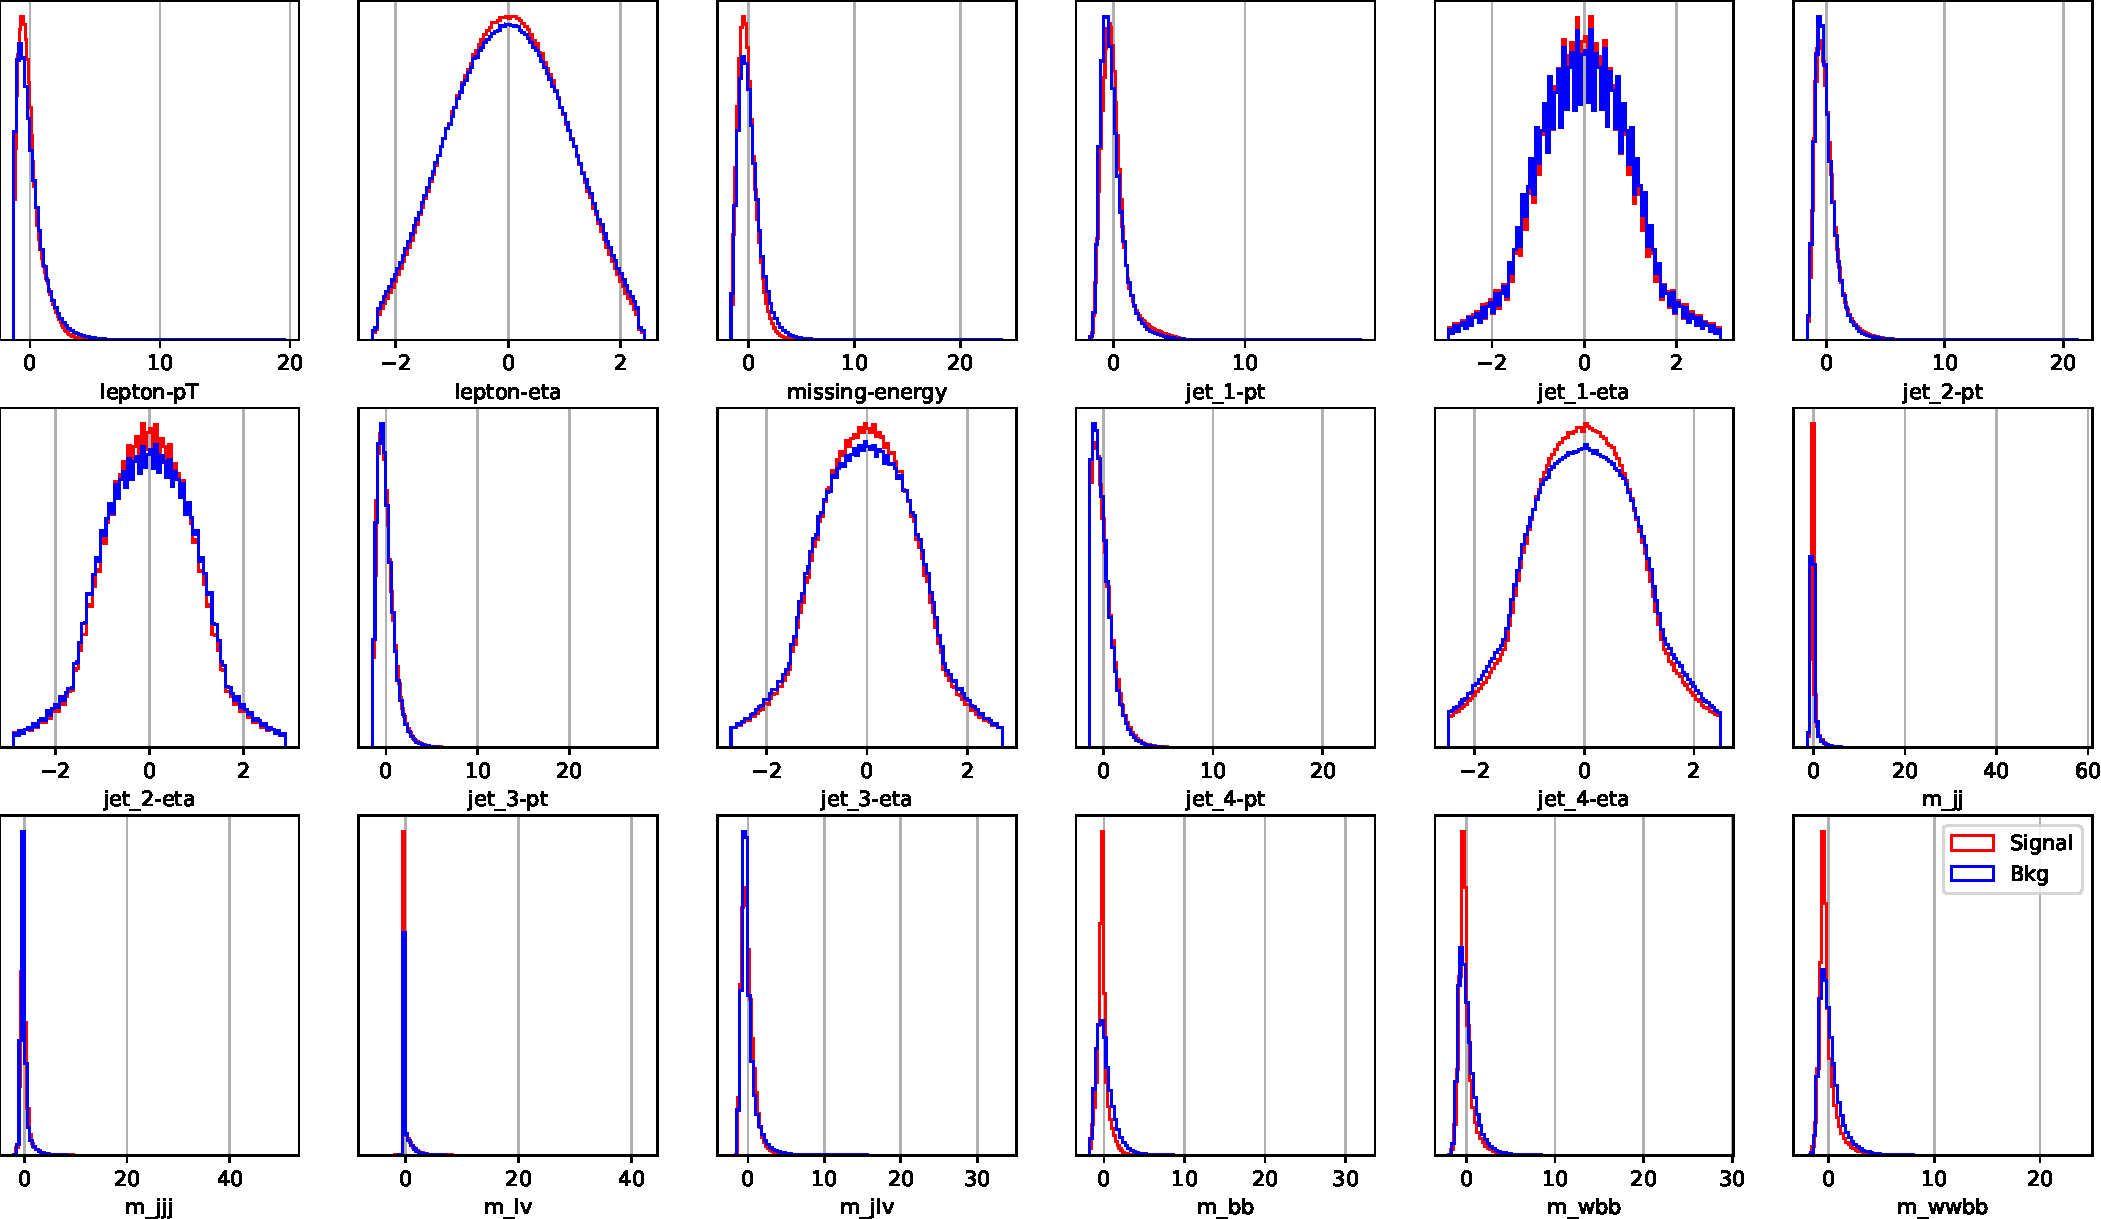
\includegraphics[width=0.95\textwidth]{../pdf/dist-sig-bkg.pdf}
    \caption{Porazdelitev signala in šuma glede na brezdimenzisko reskalirano x-os.\label{fig:dist-sig-bkg}}
\end{figure}


S pomočjo catboost knjižnjice si poglejmo kako se se spreminja natačnost modela glede na maksimalno število dreves in nekaterih drugih parametrov.
\begin{figure}[h]
    \centering
    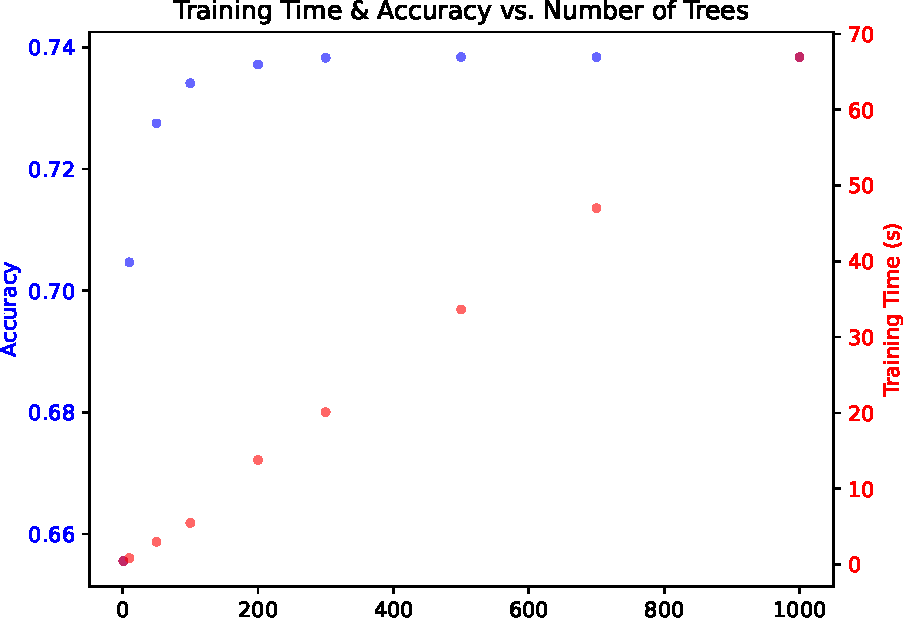
\includegraphics[width=0.45\textwidth]{../pdf/catboost_trees_vs_time_accuracy.pdf}
    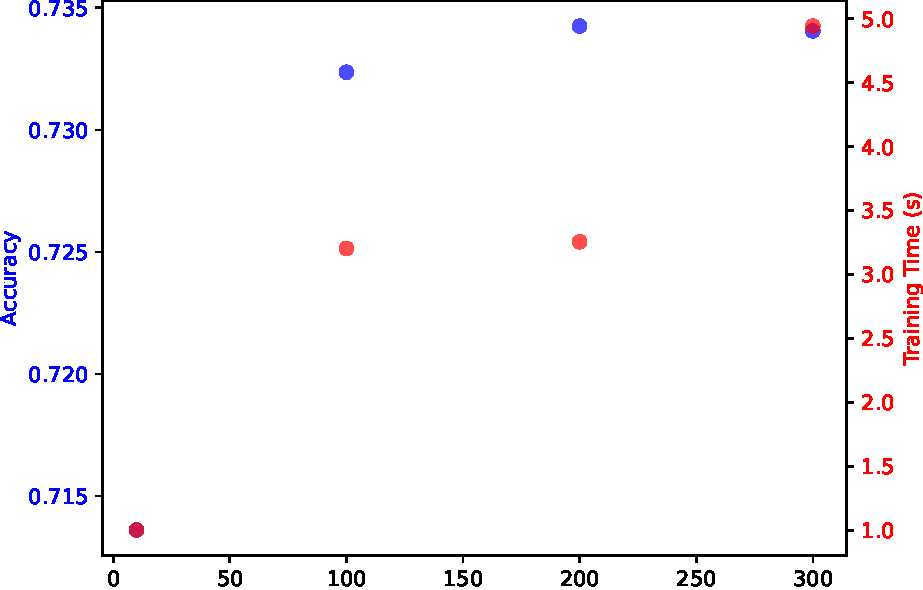
\includegraphics[width=0.45\textwidth]{../pdf/itter_time.pdf}
    \caption{Natačnost modela glede na število dreves prva slika, na drugi sliki pa je y odvisna od maksimalnega števila iteracij\label{fig:catboost-accuracy}}
\end{figure}


Poglejmo si še vpliv velikosti vhodnih podatkov na natančnost modela.
\begin{figure}
    \centering
    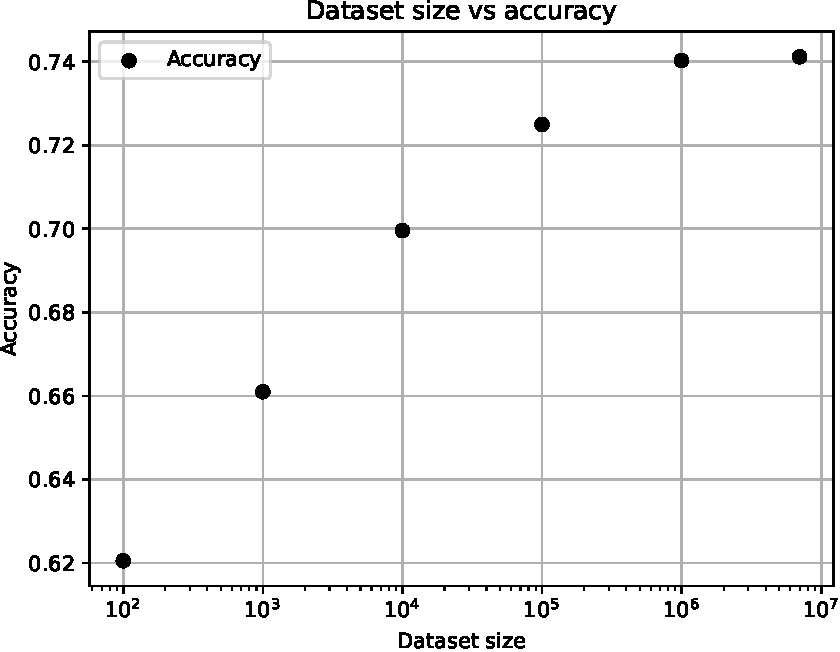
\includegraphics[width=0.45\textwidth]{../pdf/model_accuracy_vs_data_size.pdf}
    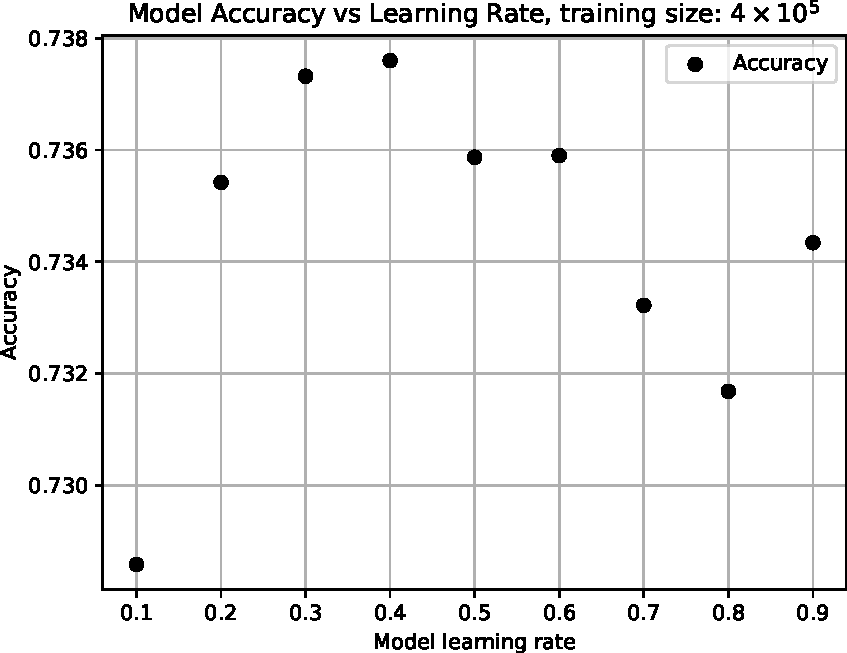
\includegraphics[width=0.45\textwidth]{../pdf/model_accuracy_vs_learning_rate.pdf}
    \caption{Natačnost modela glede na velikost vhodnih podatkov prva slika, na drugi sliki pa je y odvisna od stopnje učenja\label{fig:catboost-size}}
\end{figure}


Kaj se zgodi, če učimo na parametrih, ki bolj očitno ločujejo signal in šum?
\begin{figure}
    \centering
    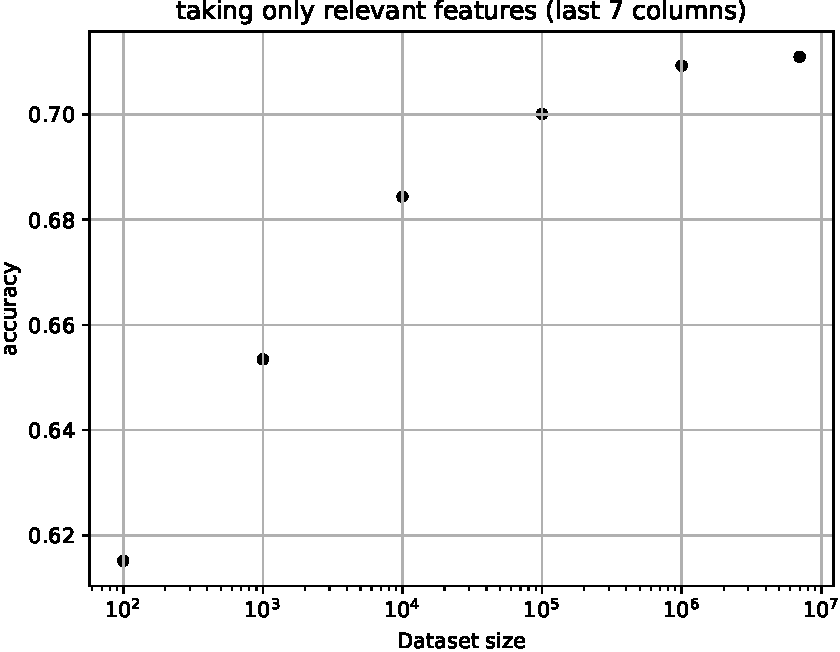
\includegraphics[width=0.7\textwidth]{../pdf/catboost_mse_vs_size.pdf}
    \caption{Uporabljenih zadnjih 7 parametrov, ki bolj očitno ločujejo signal in šum.\label{fig:catboost-mse}}
\end{figure}
\newpage
Narišemo še ROC kirvuljo pri 2 različnih velikostih vhodnih podatkov.
\begin{figure}
    \centering
    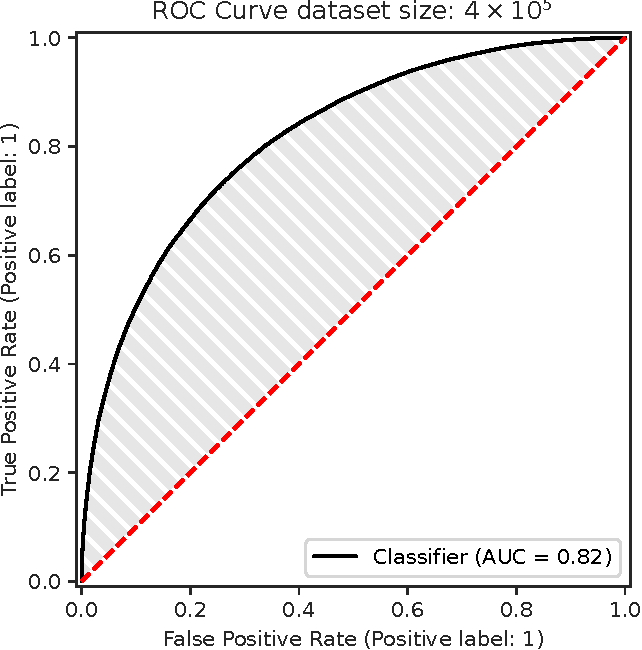
\includegraphics[width=0.45\textwidth]{../pdf/roc_boost.pdf}
    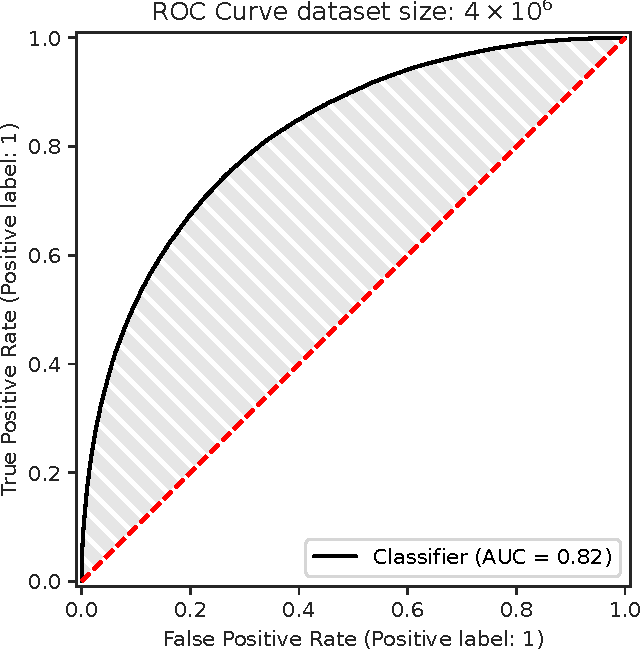
\includegraphics[width=0.45\textwidth]{../pdf/roc_boost_bigdata.pdf}
    \caption{ROC krivulja pri 2 različnih velikostih vhodnih podatkov.\label{fig:catboost-roc}}
\end{figure}

Poglejmo si še kako se obnašajo nevronske mreže.
\begin{figure}
    \centering
    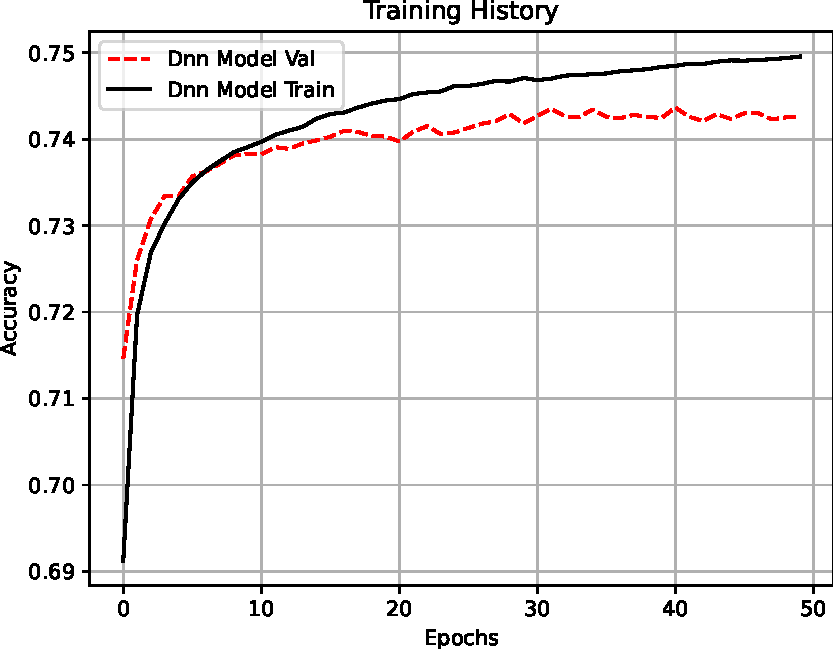
\includegraphics[width=0.40\textwidth]{../pdf/nn/training_history-accuracy.pdf}
    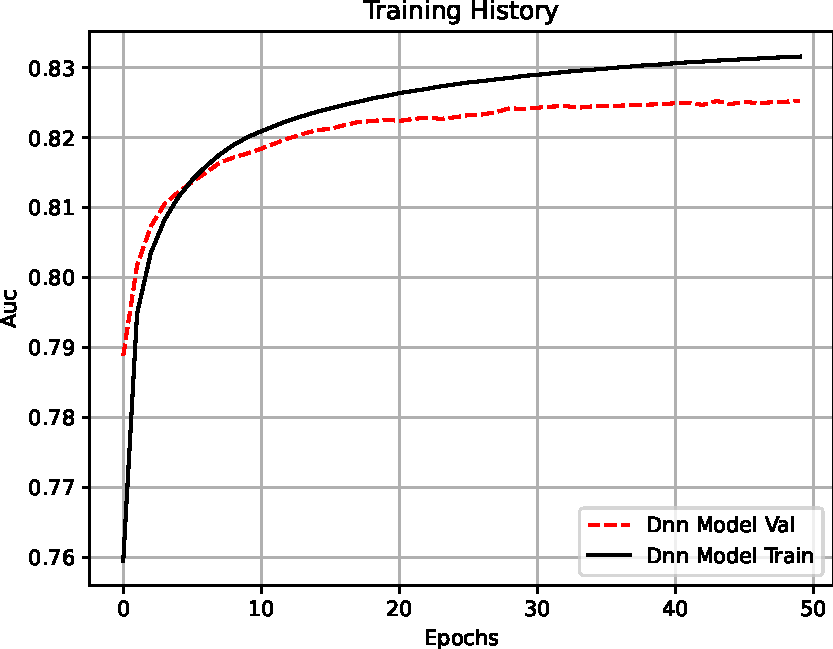
\includegraphics[width=0.40\textwidth]{../pdf/nn/training_history-AUC.pdf}
    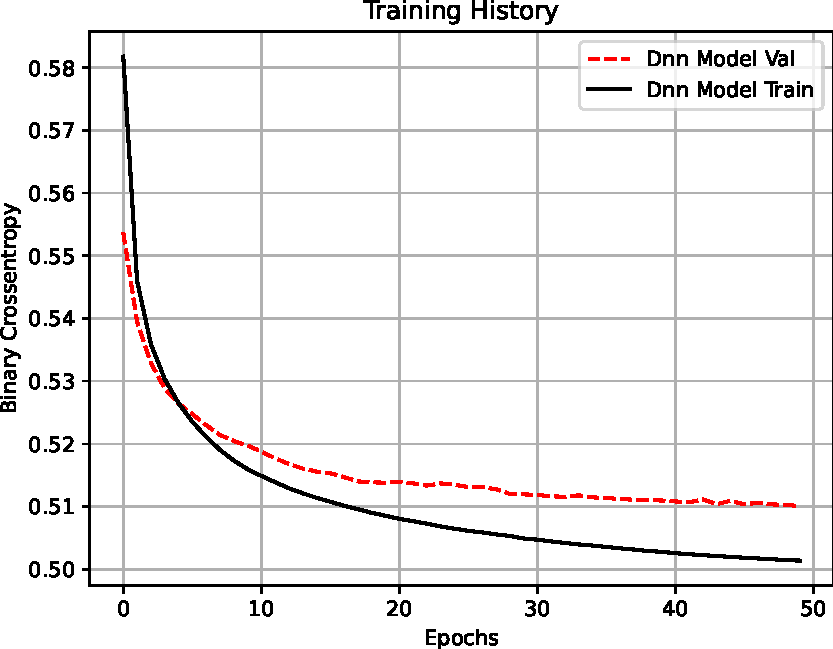
\includegraphics[width=0.40\textwidth]{../pdf/nn/training_history-binary_crossentropy.pdf}
    \caption{Natačnost in izguba nevronske mreže glede na število iteracij.\label{fig:nn-accuracy-loss}}
\end{figure}

Poglejmo si še ROC krivuljo in odziv na signal in na šum.
\begin{figure}
    \centering
    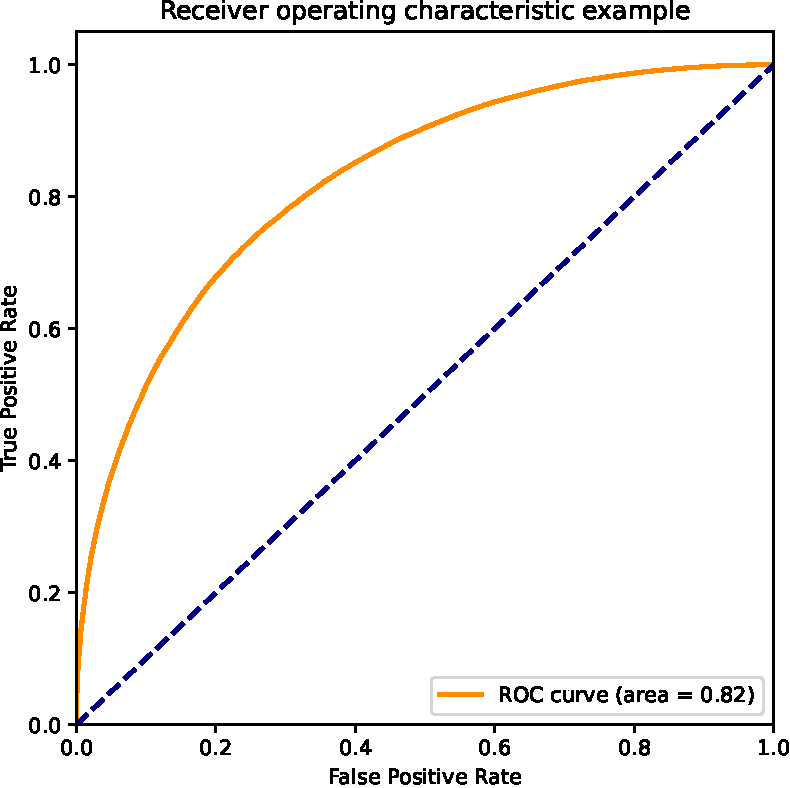
\includegraphics[width=0.45\textwidth]{../pdf/nn/roc-curve.pdf}
    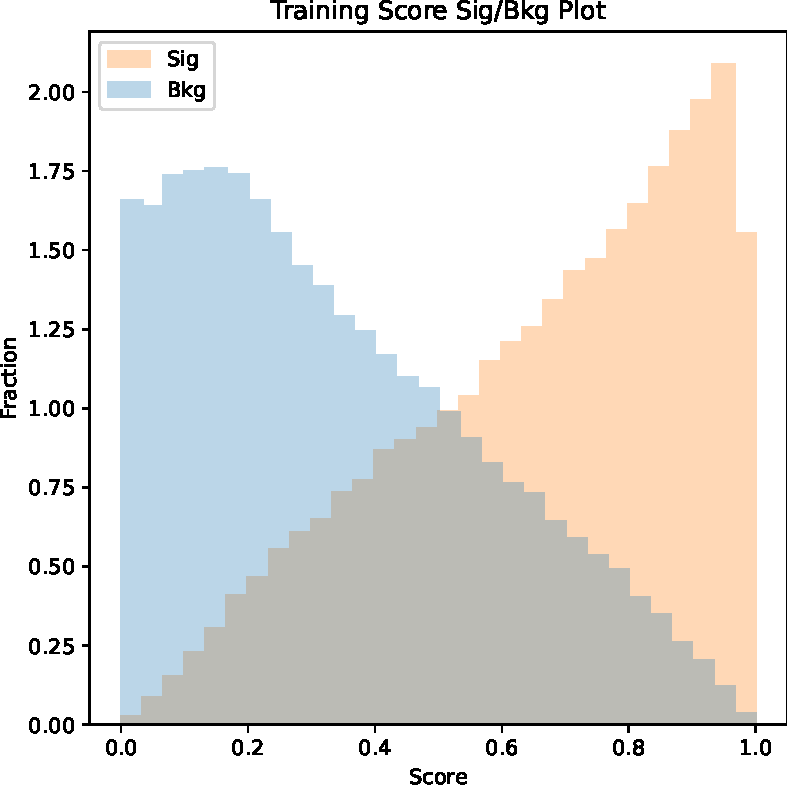
\includegraphics[width=0.45\textwidth]{../pdf/nn/ml-score.pdf}
    \caption{ROC krivulja in odziv na signal in šum.\label{fig:nn-roc-score}}
\end{figure}

Zadnji graf pa prikazuje odvisnost števila nevronov in števila skritih plasti na natančnost modela.
\begin{figure}
    \centering
    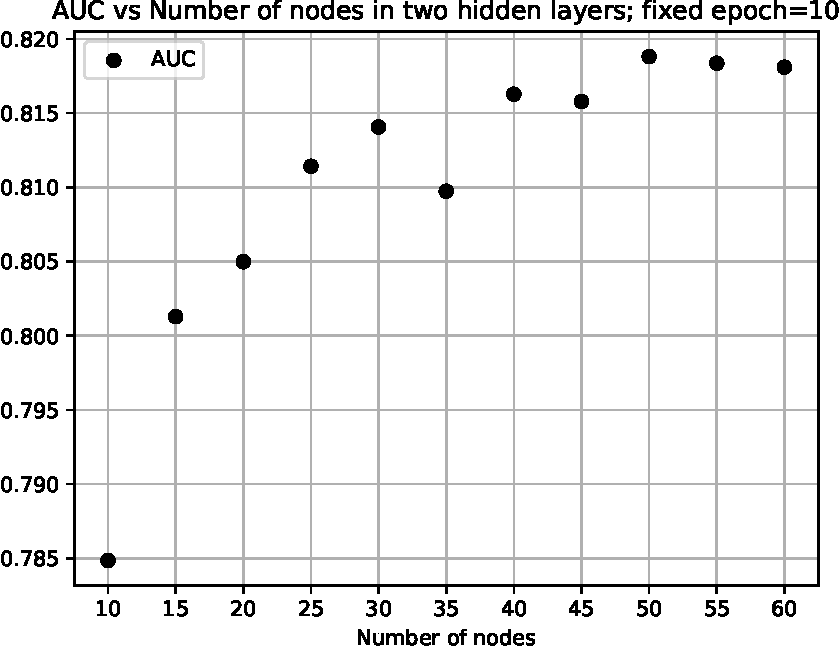
\includegraphics[width=0.45\textwidth]{../pdf/nn/auc_vs_nodes.pdf}
    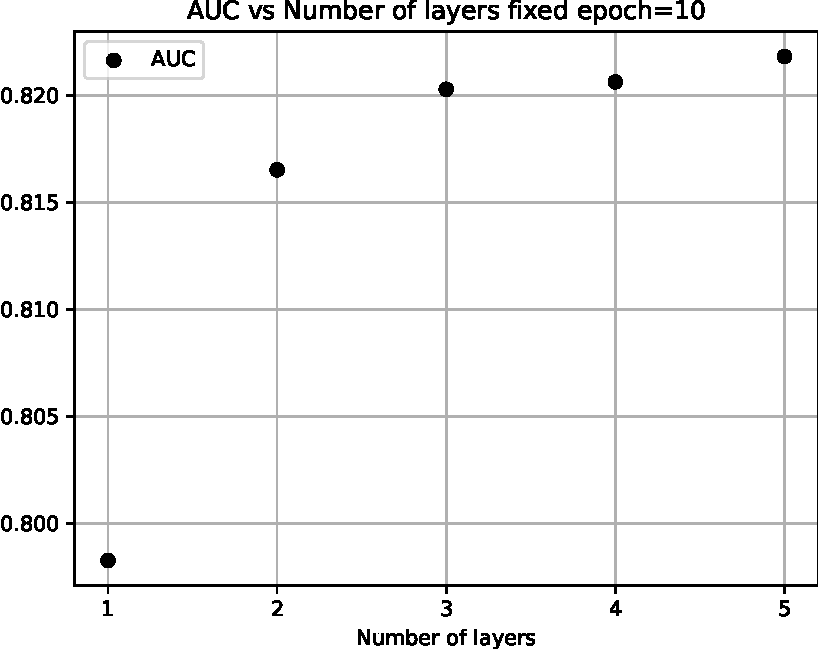
\includegraphics[width=0.45\textwidth]{../pdf/nn/auc_vs_layers.pdf}
    \caption{Odvisnost števila nevronov in števila skritih plasti na natančnost modela.\label{fig:nn-nodes-layers}}
\end{figure}
\newpage
Poglejmo si še kako močne so povezave med skritimi plastmi.
\begin{figure}
    \centering
    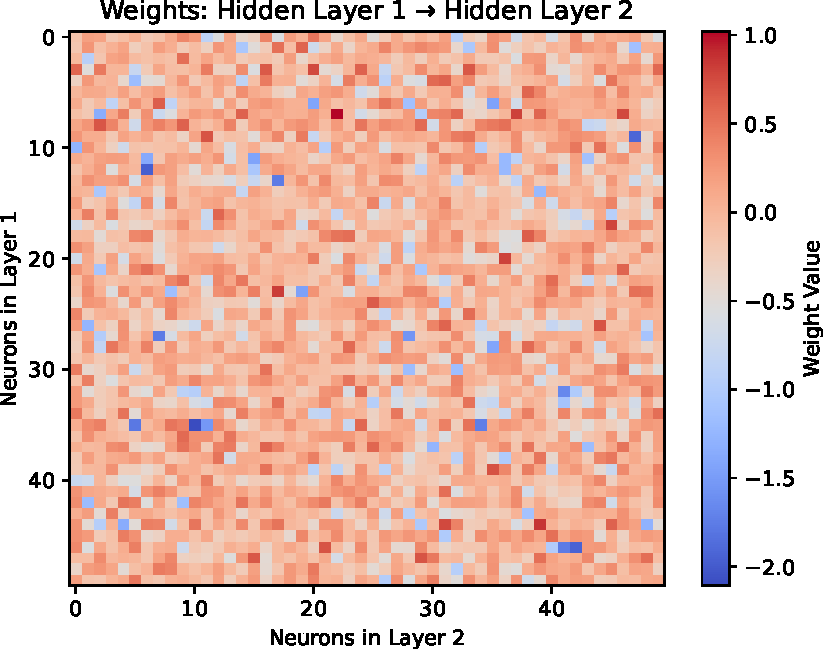
\includegraphics[width=0.45\textwidth]{../pdf/nn/weights_heatmap.pdf}
    \caption{Moč povezav med skritimi plastmi.\label{fig:nn-weights}}
\end{figure}